\subsection{Qualità di processo - Fornitura}

\vspace{0.3cm}

\subsubsection{M1PMS - Percentuale di Metriche Soddisfatte}
\begin{figure}[H]
    \centering
    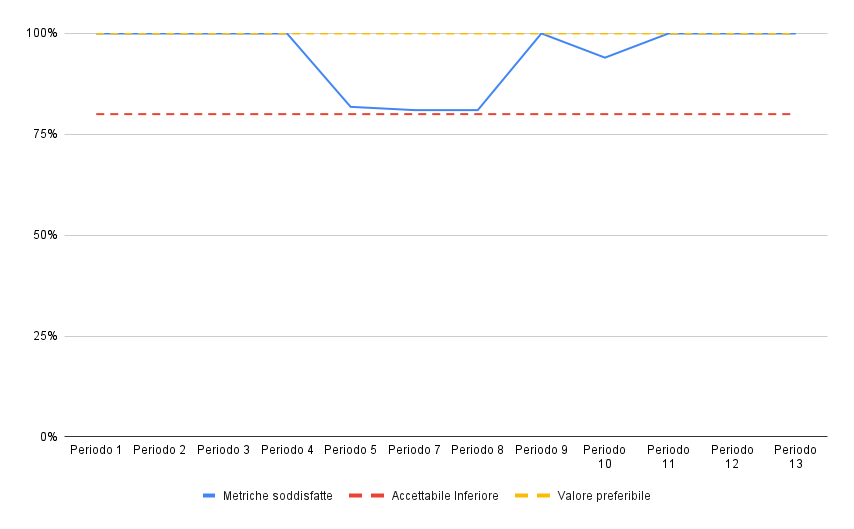
\includegraphics[width=1\textwidth]{../Images/PianoDiQualifica/M1PMS.png}
    \caption{Proiezione della percentuale di metriche soddisfatte nei vari periodi di progetto.}
    \label{fig:1}
\end{figure}

\vspace{0.2cm}

\textbf{RTB}: nel corso dei primi periodi, è evidente l'adozione di tutte le metriche di qualità; tuttavia, è solamente nell'ultimo periodo che si osserva il superamento dei valori di accettazione per due metriche, M2EAC e M4BV, fenomeno attribuibile al periodo di esami universitari.

\subsubsection{M2EAC - Estimed at Completion}

\vspace{0.3cm}

\begin{figure}[H]
    \centering
    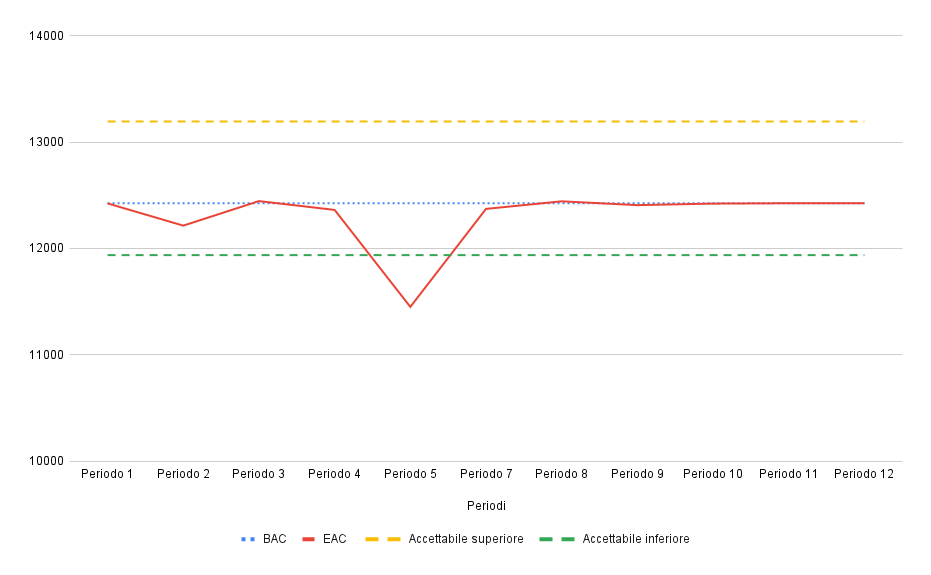
\includegraphics[width=1\textwidth]{../Images/PianoDiQualifica/M2EAC.png}
    \caption{Proiezione della stima del costo totale nei vari periodi di progetto.}
    \label{fig:2}
\end{figure}

\vspace{0.2cm}

\textbf{RTB}: si nota come nei primi periodi la stima del costo totale sia in linea con il budget inzialmente preventivato.

Tuttavia al quinto periodo, periodo di sessione degli esami, il costo totale è di molto inferiore al budget preventivato.

\vspace{0.2cm}

Questo è dovuto al fatto che in quel periodo c'è stato un calo di \textit{attività}\textsubscript{\textit{G}}, in quanto i membri del gruppo erano impegnati con gli esami universitari. Le \textit{attività}\textsubscript{\textit{G}} però rimanenti sono state completate con un costo inferiore a quello preventivato e questo ha portato ad una riduzione del costo totale.\\

\subsubsection{M7EV- Earned Value + M8PV - Planned Value} 

\vspace{0.3cm}

\begin{figure}[H]
    \centering
    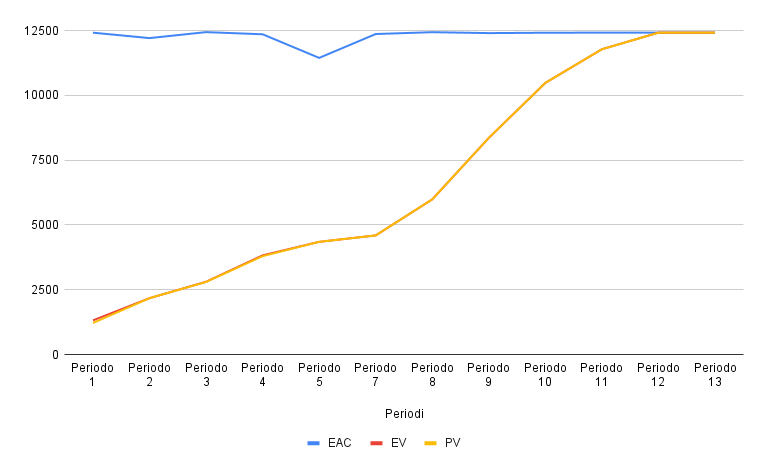
\includegraphics[width=1\textwidth]{../Images/PianoDiQualifica/EV_PV.png}
    \caption{Proiezione dell’EV e del PV nei vari periodi di progetto.}
    \label{fig:3}
\end{figure}

\vspace{0.2cm}

\textbf{RTB}: dall'analisi del grafico, è chiaro che le curve del valore guadagnato (Earned Value) e del valore pianificato (Planned Value) si sovrappongono, suggerendo che il lavoro effettivamente completato corrisponde alla pianificazione. 

\vspace{0.2cm}

Questa coincidenza implica un progresso positivo rispetto alla pianificazione del progetto.

\subsubsection{M5AC - Actual Cost + M9ETC - Estimate to Complete}

\vspace{0.3cm}

\begin{figure}[H]
    \centering
    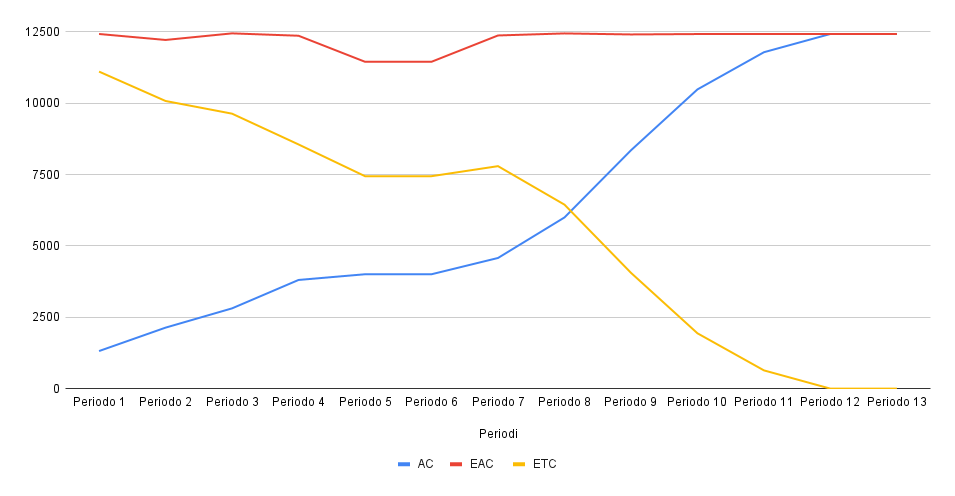
\includegraphics[width=1\textwidth]{../Images/PianoDiQualifica/AC_ETC.png}
    \caption{Proiezione dell’AC e dell’ETC nei vari periodi di progetto.}
    \label{fig:4}
\end{figure}

\vspace{0.2cm}

\textbf{RTB}: il grafico illustra l'Actual Cost (AC), che rappresenta i costi effettivamente sostenuti fino al periodo corrente per il lavoro eseguito, e l'Estimate to Complete (\textit{ETC}\textsubscript{\textit{G}}), che denota la stima dei costi rimanenti per completare il progetto durante i vari periodi.

\vspace{0.2cm}

Si osserva che l'\textit{ETC}\textsubscript{\textit{G}} tende a diminuire, come atteso, mentre l'AC mostra un incremento proporzionale alla riduzione dell'\textit{ETC}\textsubscript{\textit{G}}.

\subsubsection{M4BV - Budget Variance + M6SV - Schedule Variance}

\vspace{0.3cm}

\begin{figure}[H]
    \centering
    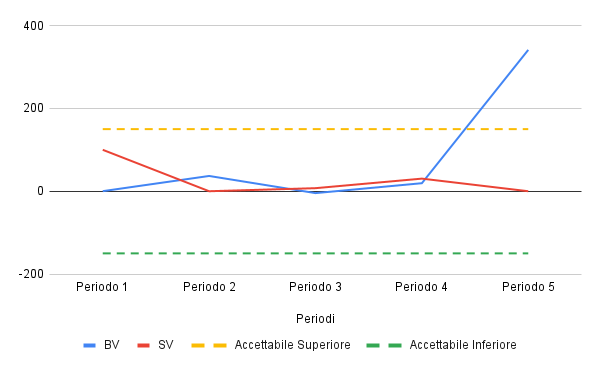
\includegraphics[width=1\textwidth]{../Images/PianoDiQualifica/BV_SV.png}
    \caption{Proiezione della BV e della SV nei vari periodi di progetto.}
    \label{fig:5}
\end{figure}

\vspace{0.2cm}

\textbf{RTB}: il grafico mostra l'andamento della Budget Variance \textit{(BV)} rappresentante la differenza tra il valore guadagnato \textit{(EV)} e i costi sostenuti \textit{(AC)} e la Schedule Variance \textit{(SV)} che indica la differenza tra il valore guadagnato \textit{(EV)} e il valore pianificato (\textit{PV}\textsubscript{\textit{G}}).

\vspace{0.2cm}

Si nota come la Budget Variance sia sempre diversa da zero, suggerendo che ad ogni periodo, tranne il primo dove abbiamo un valore molto vicino a zero, ci sia una discrepanza dal costo preventivato a quello effettivo fino al periodo di riferimento. 

\vspace{0.2cm}

Nell'ultimo periodo si nota un grande aumento della Budget Variance, questo è dovuto al fatto che le \textit{attività}\textsubscript{\textit{G}} rimanenti sono state completate con un costo inferiore a quello preventivato. 
Risulta anche altalenante la Schedule Variance, indicando che in ogni periodo ci sono stati dei ritardi o degli anticipi rispetto alla pianificazione.

\vspace{0.2cm}

Nell'ultimo periodo si è raggiunto l'ottimo per la Schedule Variance. 

\subsubsection{M3CPI - Cost Performance Index}

\vspace{0.3cm}

\begin{figure}[H]
    \centering
    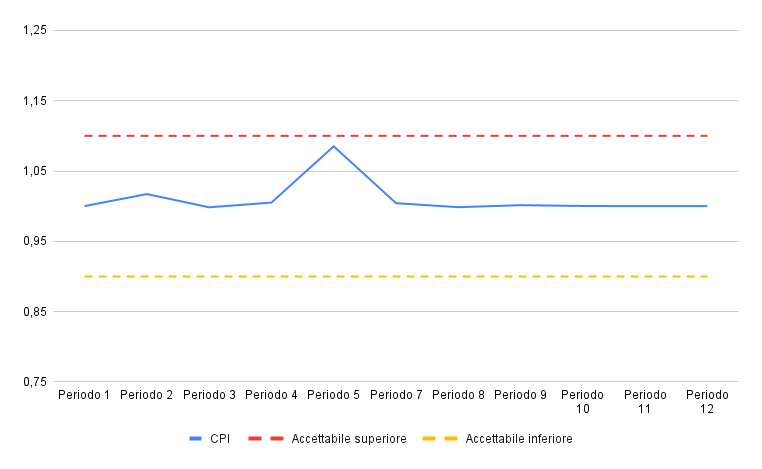
\includegraphics[width=1\textwidth]{../Images/PianoDiQualifica/M3CPI.png}
    \caption{Proiezione del CPI nei vari periodi di progetto.}
    \label{fig:6}
\end{figure}

\vspace{0.2cm}

\textbf{RTB}: il grafico evidenzia la costante prossimità del nostro Cost Performance Index (\textit{CPI}\textsubscript{\textit{G}}) a 1, suggerendo che il progetto stia mantenendo i costi in linea con la pianificazione.

\vspace{0.2cm}

In particolare, nell'ultimo periodo, si osserva un incremento del \textit{CPI}\textsubscript{\textit{G}}, indicando che le \textit{attività}\textsubscript{\textit{G}} rimanenti sono state completate con un costo inferiore rispetto a quanto inizialmente previsto.

\subsubsection{M11RNP - Rischi non previsti}

\vspace{0.3cm}

\begin{figure}[H]
    \centering
    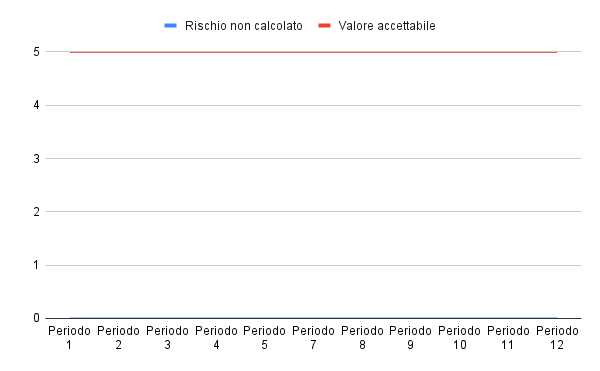
\includegraphics[width=1\textwidth]{../Images/PianoDiQualifica/M11RNP.png}
    \caption{Proiezione rischi non previsti nei vari periodi di progetto.}
    \label{fig:7}
\end{figure}

\vspace{0.2cm}

\textbf{RTB}: il grafico mostra come i rischi non previsti siano rimasti costanti durante tutto il progetto. Questo è un buon segno, in quanto indica che il gruppo è stato in grado di gestire i rischi in modo efficace e che non sono emersi nuovi rischi inaspettati.
